\documentclass[11pt]{article}

\usepackage[a4paper,margin=1in]{geometry}
\usepackage{amsmath,amssymb}
\usepackage{graphicx}
\usepackage{booktabs}
\usepackage{caption}
\usepackage{hyperref}
\usepackage{xcolor}

\graphicspath{{../results/}}
\hypersetup{colorlinks=true, linkcolor=blue!50!black, urlcolor=blue!50!black}

\title{Learning a Cumulative Distribution Function with a Neural Network,\\
Trained on a Kernel-Density Estimate}
\author{Univariate experiments (Step 1)}
\date{\today}

\newcommand{\Fhat}{\widehat{F}}
\newcommand{\fhat}{\widehat{f}}

\begin{document}
\maketitle

\begin{abstract}
We study a small pipeline for estimating a probability distribution from samples. From data drawn
from a \emph{known} distribution we build a smooth, closed-form estimate of its cumulative
distribution function (CDF), then train a neural network to reproduce that estimate, and finally read
the probability density off the trained network as its derivative. Because the data comes from a
known distribution, we can score every estimate against the exact truth. This report is
self-contained: it defines each ingredient, then narrates the experiments run so far --- a naive
baseline, a deep study on a single Gaussian, and a study on two simple mixtures --- and states what
we learned. The headline result is that, once trained properly, \textbf{the network faithfully
reproduces the kernel estimate it is trained on but does not by itself surpass it}; the largest
accuracy gain comes from a better, fully data-driven choice of the kernel's smoothing width. We close
with the open question this raises and the techniques that could answer it.
\end{abstract}

\tableofcontents

\section{The problem and the idea}

We are given samples $x_1,\dots,x_n$ drawn independently from some distribution, and we want to
estimate that distribution: both its \textbf{cumulative distribution function} (CDF)
$F(x) = \Pr[X \le x]$ --- a curve that rises monotonically from $0$ to $1$ --- and its
\textbf{probability density function} (the density, or pdf) $f(x) = F'(x)$.

The experimental trick is to use \emph{synthetic} data from a \emph{known} distribution, specifically
a mixture of Gaussians (a weighted sum of bell curves). A Gaussian mixture has a known density, a
known CDF, and an exact sampler, so any estimate we produce can be compared against the exact truth.

The pipeline, in plain terms:
\begin{enumerate}
  \item \textbf{Choose} a known Gaussian mixture.
  \item \textbf{Sample} $n$ points from it.
  \item \textbf{Smooth-estimate the CDF} from those points with a kernel method (Section~\ref{sec:parzen}),
  giving a smooth closed-form curve $\Fhat$.
  \item \textbf{Train a neural network} to reproduce $\Fhat$, using the network's output as an
  estimate of the \emph{true} CDF.
  \item \textbf{Recover the density} as the derivative of the trained network.
\end{enumerate}

\paragraph{Why involve a neural network at all, if the kernel method already gives a CDF?} This is a
fair question and part of what the experiments probe. The hoped-for payoffs are: a compact,
differentiable functional form (so the density comes for free by differentiation); the possibility
that the network's built-in smoothness \emph{denoises} the finite-sample kernel estimate and lands
closer to the truth than the estimate it is trained on; and a path to higher dimensions later.
Whether the network actually delivers the first two is something we test, not assume.

\paragraph{The rule that defines this project.} The network is trained \textbf{only on the $n$ sample
points}, each labelled with the kernel estimate's value there. We do not invent extra input points,
we do not query the kernel estimate anywhere except at the data, and we do not augment the data in any
way. This is a deliberate, strict honesty constraint: the network sees exactly the data and nothing
more. (The dense grids that appear later are used only for \emph{scoring} against the truth, never for
training.)

\section{The building blocks}
\label{sec:parzen}

\subsection{The kernel estimate of the CDF}

A kernel density estimate (also called a Parzen-window estimate) places a small bump --- a
\emph{kernel} --- on each data point and sums them. We use a \textbf{logistic kernel}, chosen for one
convenient property: the integral of the logistic bump is the logistic S-curve
$\sigma(z) = 1/(1+e^{-z})$. That makes the estimated CDF available in closed form as an average of
S-curves, and the density is its exact derivative:
\begin{equation}
  \Fhat(x) = \frac{1}{n}\sum_{i=1}^{n}\sigma\!\Big(\frac{x-x_i}{h}\Big),
  \qquad
  \fhat(x) = \frac{1}{n}\sum_{i=1}^{n}\frac{1}{h}\,\sigma(z_i)\,\big(1-\sigma(z_i)\big),
  \quad z_i = \frac{x-x_i}{h}.
\end{equation}
Here $h>0$ is the \textbf{bandwidth}: the width of each bump. A small $h$ gives a sharp, wiggly
estimate; a large $h$ gives a smooth, blurry one. Choosing $h$ well is the central tuning problem of
kernel estimation.

\subsection{Ways to choose the bandwidth (all data-driven)}

Every rule below uses only the samples --- none peeks at the truth --- so each is something one could
actually deploy.
\begin{itemize}
  \item \textbf{Silverman's rule}: a standard closed-form default, $h \propto n^{-1/5}$ times a
  spread estimate. Simple, but tuned for a single bell-shaped distribution, so it tends to
  over-smooth distributions with several peaks.
  \item \textbf{Variance-matched}: Silverman's rule rescaled so the (wider) logistic kernel smooths
  like the bell-shaped kernel Silverman was designed for --- a principled shrink of $h$.
  \item \textbf{Cross-validation}: pick $h$ by leaving each point out and asking which $h$ best
  predicts the held-out points. Two variants: a likelihood criterion and a least-squares criterion.
  \item \textbf{Adaptive (per-point) bandwidth}: use a \emph{narrower} bump where data is dense and a
  \emph{wider} one in sparse tails, instead of one global $h$. Good for distributions whose features
  live at different scales.
\end{itemize}

\subsection{The neural network}

The network is a small \textbf{multilayer perceptron}: a few layers of weighted sums separated by a
smooth S-shaped activation, mapping a scalar $x$ to a value in $(0,1)$ via a final S-curve (so the
output has the range of a CDF). We require \emph{smooth} activations because the density is obtained
by differentiating the output; a kink in the network would put a discontinuity in the density.

A CDF must never decrease. We consider three ways to enforce this:
\begin{itemize}
  \item \textbf{A penalty} that punishes any downward slope of the network output during training;
  \item \textbf{Monotone-by-construction}: forcing every weight to be non-negative (via a smooth
  positive reparameterisation) so the network is automatically non-decreasing --- we call this the
  \emph{constrained} network;
  \item \textbf{After-the-fact correction}: rectify a trained curve to be non-decreasing.
\end{itemize}

\subsection{The scorecard}

\begin{itemize}
  \item \textbf{CDF gap} (Kolmogorov--Smirnov distance): the single largest vertical gap between the
  estimated CDF and the true CDF. One number; smaller is better. We write it as ``CDF gap''.
  \item \textbf{Density error}: mean squared error between the estimated and true density.
  \item \textbf{Monotonicity violations}: the fraction of the curve that goes downhill (should be $0$).
  \item \textbf{Recovered mass}: the integral of the estimated density (should be $1$).
\end{itemize}

\paragraph{The ``kernel ceiling''.} Because the network is trained to copy the kernel estimate
$\Fhat$, the kernel estimate's own gap to the truth is the network's target --- and, in the ordinary
case, the best it can be expected to do. Throughout, we report this kernel ceiling alongside the
network so the reader can see how close the network gets, and whether it ever does better.

\section{The experiments}

All experiments train only on the data points, score against the known truth on a dense grid, and use
a fixed random seed for reproducibility. We vary one setting at a time off a baseline.

\subsection{First attempt: a naive baseline}

We start as simply as possible: a one-hidden-layer network of width $16$, a modest learning rate
($0.01$) and training length ($2000$ steps), Silverman's bandwidth, $n=2000$ samples, on all four of
our distributions at once. The network learns a sensible CDF, but the recovered density is a single
smooth bump that misses any multi-peak structure (Figure~\ref{fig:naive}). Two problems are stacked:
the small network is \emph{under-trained}, and the Silverman bandwidth has \emph{over-smoothed} the
target it is being trained to copy. This motivates studying the knobs deliberately, one distribution
at a time, starting from the simplest.

\begin{figure}[h]
  \centering
  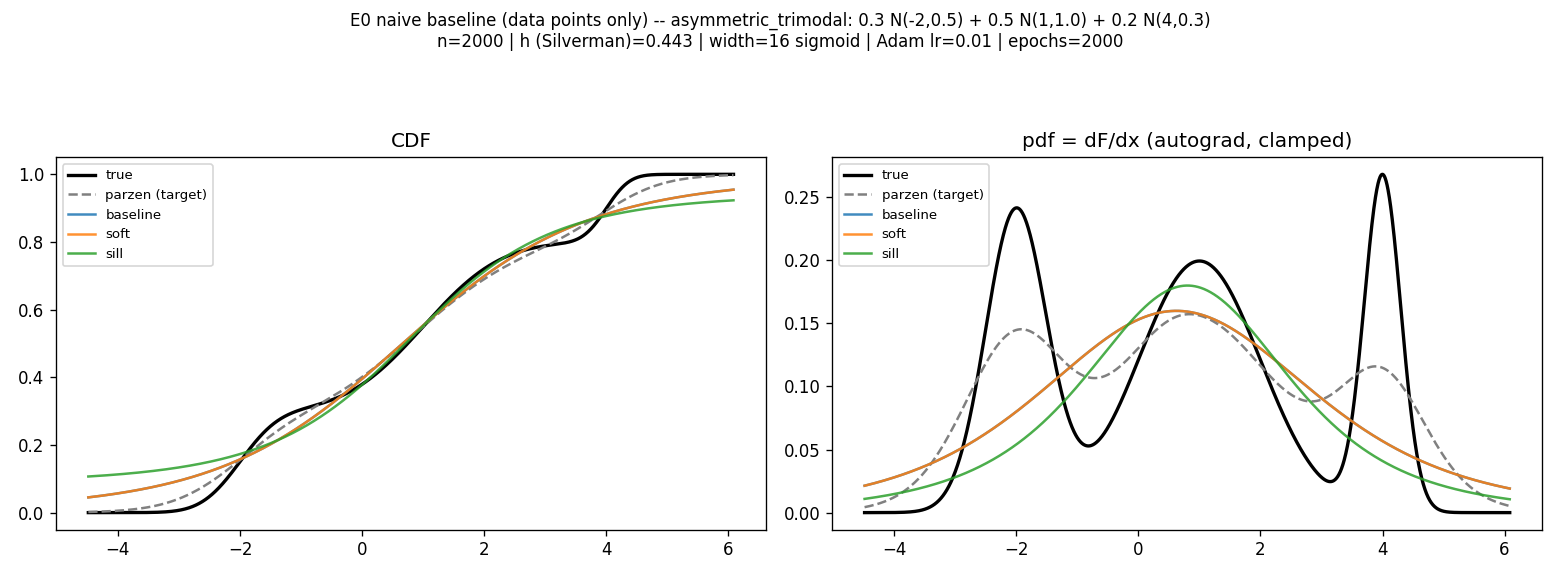
\includegraphics[width=\textwidth]{e0_naive_asymmetric_trimodal.png}
  \caption{The naive baseline on a three-peak mixture. Left: CDF; right: density. Black is the truth,
  gray dashed is the kernel estimate the network is trained to copy, coloured curves are the network
  (three monotonicity strategies). The network under-fits to a single bump, and the kernel target
  itself is too smooth to show the three peaks.}
  \label{fig:naive}
\end{figure}

\subsection{A deep study on the single Gaussian}

We take the simplest possible target --- a standard bell curve --- and vary each knob in turn off the
naive baseline, with no multi-peak structure to confuse the picture. The kernel ceiling here is a CDF
gap of $0.020$.

\begin{table}[h]
  \centering
  \caption{Single Gaussian: CDF gap (smaller is better) as each knob varies; the kernel ceiling is
  $0.020$. ``Recovered mass'' should be $1$. One knob varies per block.}
  \small
  \begin{tabular}{llcc}
    \toprule
    Knob & Setting & CDF gap & Recovered mass \\
    \midrule
    Network size (width)   & $16$           & 0.032 & 0.99 \\
                           & $128$          & 0.026 & 1.00 \\
                           & two layers, $32{+}32$ & \textbf{0.021} & 0.99 \\
                           & three layers   & 0.042 & 0.99 \\
    \midrule
    Learning rate          & $0.001$        & 0.037 & 0.98 \\
                           & $0.01$         & 0.032 & 0.99 \\
                           & $\mathbf{0.1}$ & \textbf{0.019} & 1.00 \\
    \midrule
    Training length        & $2000$ steps   & 0.032 & 0.99 \\
                           & $\mathbf{10000}$ steps & \textbf{0.020} & 1.00 \\
    \midrule
    Bandwidth              & $0.3\times$ Silverman & 0.026 & 0.99 \\
                           & Silverman             & 0.032 & 0.99 \\
                           & $1.5\times$ Silverman & 0.041 & 0.99 \\
                           & adaptive              & \textbf{0.026} & 0.99 \\
    \midrule
    Monotonicity           & none / penalty (identical) & 0.032 & 0.99 \\
                           & constrained network        & 0.077 & 0.88 \\
    \bottomrule
  \end{tabular}
  \label{tab:gauss}
\end{table}

The story (Table~\ref{tab:gauss}, Figure~\ref{fig:gauss}):
\begin{itemize}
  \item \textbf{The naive baseline was simply under-trained.} Raising the learning rate to $0.1$, or
  training for $10000$ steps, each bring the network down to the kernel ceiling. Optimisation, not
  network size, was the limiting factor.
  \item \textbf{Network size has diminishing returns.} A wider single layer helps a little; a
  two-layer network is best; a three-layer network is actually worse, because it is harder to train in
  the same budget.
  \item \textbf{Bandwidth barely matters here.} For a single bell curve, Silverman is already close to
  ideal; a slightly narrower or adaptive bandwidth is marginally better, over-smoothing is worse.
  \item \textbf{Monotonicity costs nothing to ask for.} The unconstrained network never produces a
  decreasing CDF, so the penalty never activates (the ``none'' and ``penalty'' rows are identical).
  Forcing monotonicity by construction, by contrast, noticeably hurts accuracy and loses mass on this
  small network --- it is an unnecessary handicap on an easy problem.
\end{itemize}

\begin{figure}[h]
  \centering
  
\includegraphics[width=\textwidth]{stage_a_single_gaussian.png}
  \caption{Single-Gaussian study: CDF gap versus each knob. Gray dashed line is the kernel ceiling.
  Optimisation (learning rate, training length) moves the network down to the ceiling; the other
  knobs move it little.}
  \label{fig:gauss}
\end{figure}

\subsection{Two simple mixtures}

We now move to two two-peak distributions --- one symmetric, one lopsided --- carrying the lesson from
the single Gaussian (train properly: width $32$, learning rate $0.1$, $5000$ steps). The kernel
ceilings are CDF gaps of $0.048$ (symmetric) and $0.027$ (lopsided).

The dominant result is the bandwidth (Table~\ref{tab:bw}): switching from Silverman to a
cross-validated or adaptive bandwidth \emph{roughly halves} the CDF gap on both mixtures, while
over-smoothing makes it worse. Every other knob is comparatively flat:
\begin{itemize}
  \item Network size plateaus early --- width $8$ is already enough --- so there is no under-fitting
  once training is adequate.
  \item A learning rate of $0.001$ under-trains badly, but anything from $0.01$ upward reaches the
  ceiling. One caution: a learning rate of $0.1$ \emph{diverged} on the largest network (width $128$):
  its output collapsed, mass went to $0$. The safe rate is about $0.03$.
  \item Monotonicity is still never an issue --- zero violations --- and the constrained network is now
  roughly on par with the others (the handicap we saw on the tiny single-Gaussian network has faded at
  this larger size).
\end{itemize}

\begin{table}[h]
  \centering
  \caption{Two mixtures: CDF gap as the bandwidth rule changes (other settings fixed). A
  cross-validated or adaptive bandwidth roughly halves the gap versus Silverman. Kernel ceilings at
  Silverman: $0.048$ and $0.027$.}
  \begin{tabular}{lcc}
    \toprule
    Bandwidth rule & Symmetric mixture & Lopsided mixture \\
    \midrule
    $0.3\times$ Silverman (sharper)     & 0.020 & 0.012 \\
    Silverman (default)                 & 0.050 & 0.027 \\
    $1.5\times$ Silverman (over-smooth) & 0.069 & 0.045 \\
    variance-matched                    & 0.026 & 0.016 \\
    cross-validation (likelihood)       & 0.020 & 0.012 \\
    cross-validation (least-squares)    & 0.020 & 0.013 \\
    \textbf{adaptive (per-point)}       & \textbf{0.019} & \textbf{0.012} \\
    \bottomrule
  \end{tabular}
  \label{tab:bw}
\end{table}

\begin{figure}[h]
  \centering
  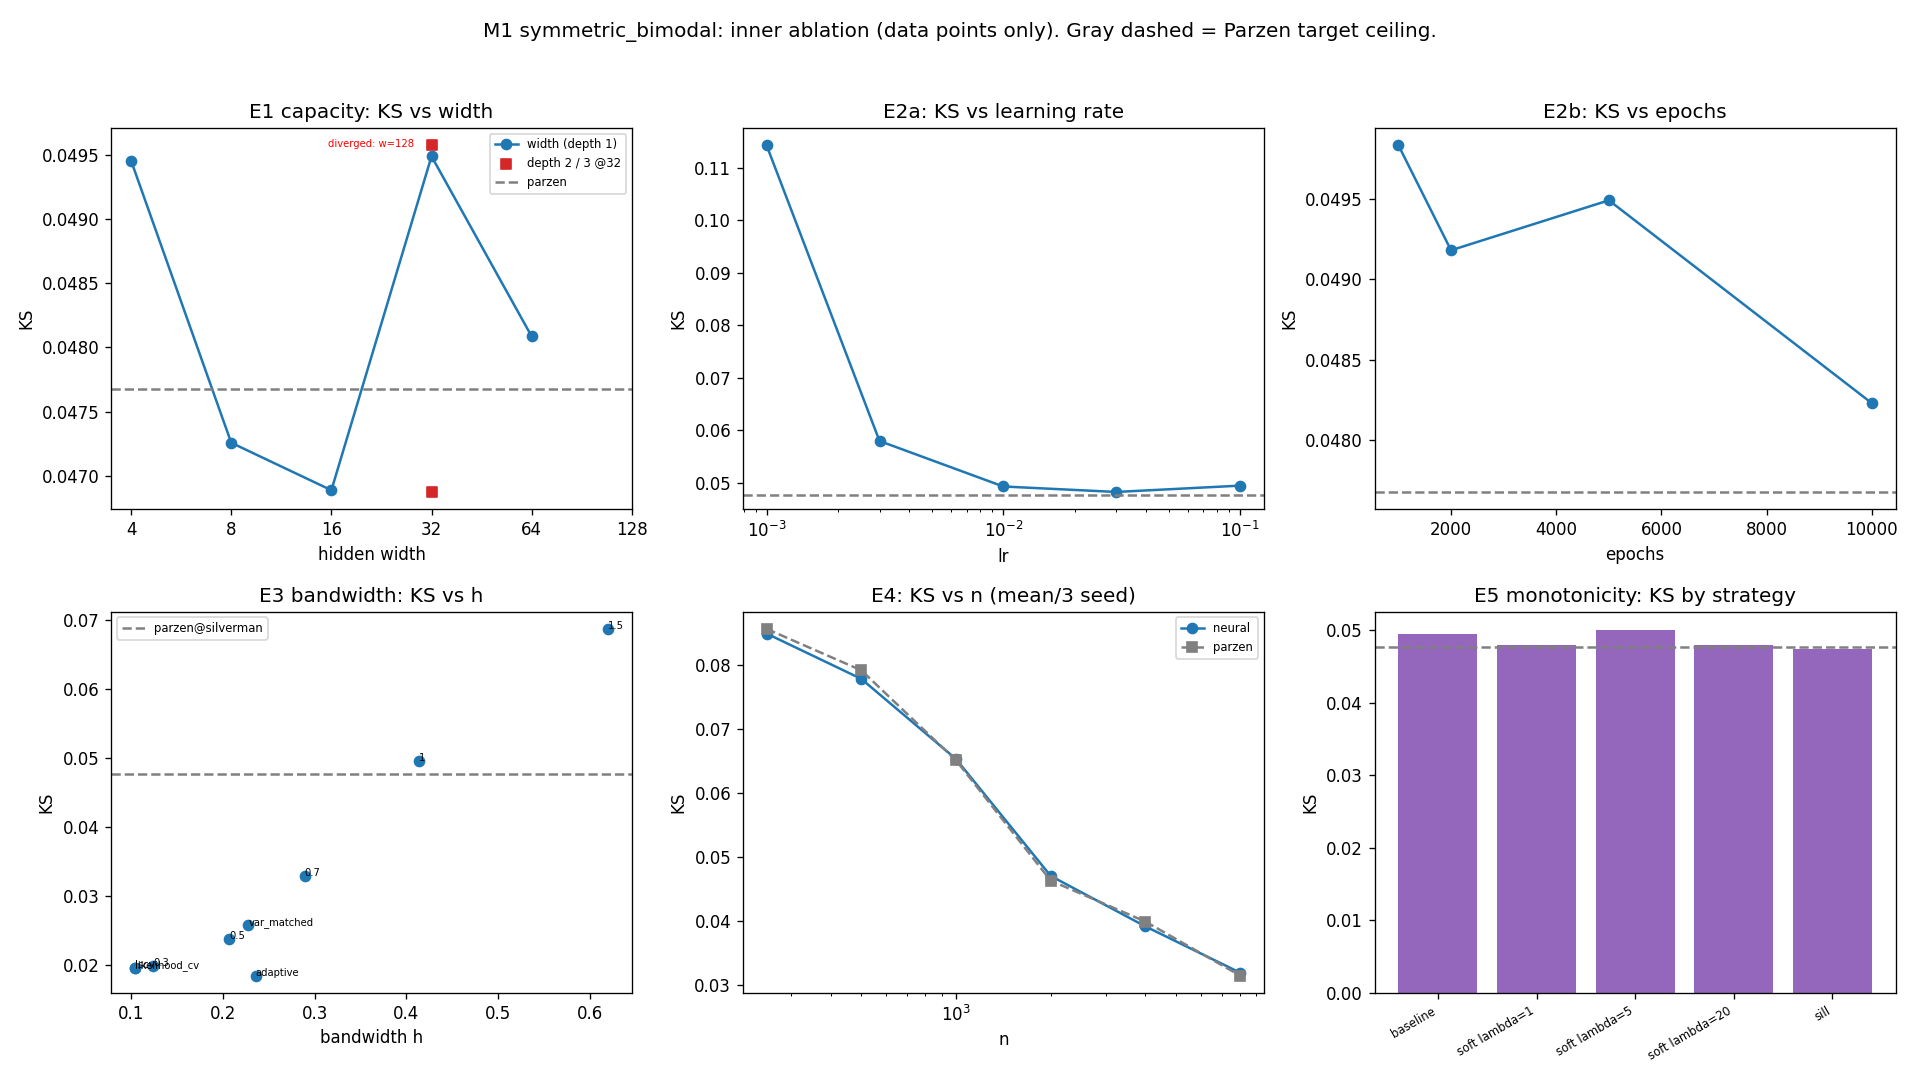
\includegraphics[width=0.49\textwidth]{stage_b_symmetric_bimodal.png}\hfill
  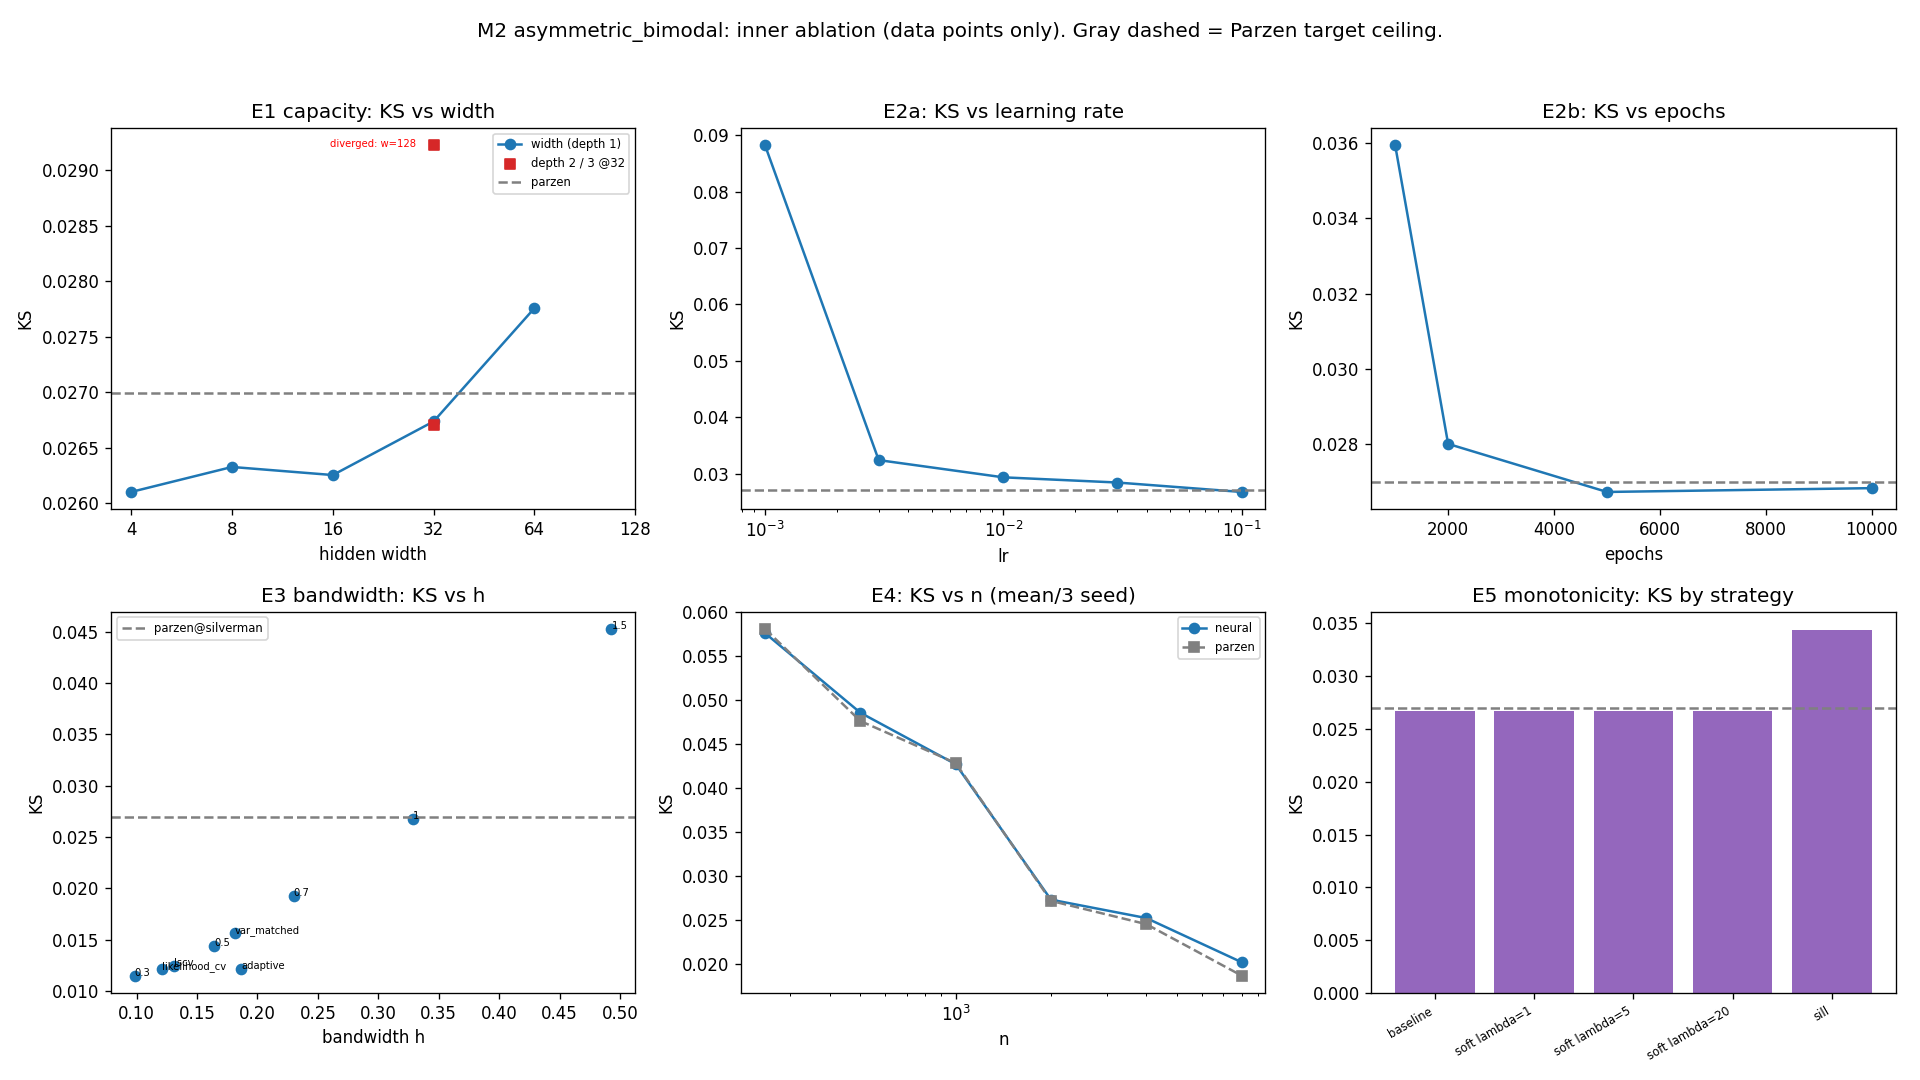
\includegraphics[width=0.49\textwidth]{stage_b_asymmetric_bimodal.png}
  \caption{The two two-peak mixtures (symmetric left, lopsided right). The bandwidth panel
  (bottom-left of each) slopes clearly downward toward sharper bandwidths; the network-size,
  learning-rate-plateau and monotonicity panels are flat. ``Diverged'' marks the width-$128$ run that
  blew up at learning rate $0.1$.}
  \label{fig:mixtures}
\end{figure}

\section{What we learned}

Two findings stand out, and they reinforce each other.

\paragraph{The network is a faithful copy of the kernel estimate.} On the two mixtures, the network's
CDF gap matches the kernel estimate's gap almost exactly --- as the sample count changes and as the
bandwidth changes, the two move together. Given adequate (but not over-aggressive) training, the
network reaches the kernel ceiling and stops there. It does not, on its own, beat the estimate it is
trained to copy.

\paragraph{So the real accuracy lever is the bandwidth, and it is data-driven.} Because the network
faithfully transmits whatever target it is given, the way to a better answer is a better target ---
and a cross-validated or adaptive bandwidth, chosen from the samples alone, roughly halves the error
over the default. Network size and the monotonicity machinery are, for these smooth distributions,
second-order.

\paragraph{An honest caveat, and a hint.} If the network only ever matches the kernel estimate, one
should ask what it adds over simply using the kernel estimate directly. There is one encouraging
hint: at small sample sizes, where the kernel estimate is noisiest, the network's gap is consistently
a touch \emph{smaller} than the kernel estimate's --- its built-in smoothness appears to denoise the
target slightly. We have not yet tried to amplify this deliberately. Doing so is the most promising
next direction (Section~\ref{sec:next}), and is more valuable than simply running more distributions.

\section{Where next}
\label{sec:next}

The experiments so far establish a solid, well-understood baseline but leave the central
value question open: \emph{can the network be made to surpass the kernel estimate, rather than merely
copy it?} The candidate techniques, all compatible with the strict training rule, are: regularising
the network toward smoothness so it fits the underlying trend rather than the finite-sample noise
(turning the faint denoising hint into a real gain); anchoring the network's boundary behaviour so the
density integrates exactly to one (it currently loses a few percent of its mass); and averaging
several networks to reduce variance. The remaining, sharper distributions (a three-peak mixture and a
narrow spike inside a broad mode) are also still to be studied, and are where network capacity and the
monotonicity constraint may finally start to matter.

\paragraph{Reproducibility.} Every figure and number above is regenerated by the scripts in
\texttt{scripts/experiments/} (\texttt{e0\_naive\_baseline.py},
\texttt{stage\_a\_single\_gaussian.py}, \texttt{stage\_b\_simple\_mixtures.py}); a fuller running log,
including the exact per-setting tables, lives in \texttt{docs/experiments.md}.

\end{document}
